\def\year{2016}\relax
%File: formatting-instruction.tex
\documentclass[letterpaper]{article}
\usepackage{aaai16}
\usepackage{times}
\usepackage{helvet}
\usepackage{courier}
\usepackage{graphicx}
\usepackage{epsfig}
\frenchspacing
\setlength{\pdfpagewidth}{8.5in}
\setlength{\pdfpageheight}{11in}
\pdfinfo{
/Title (Learning Topical Social Sensor on Twitter)
/Author (Author1, Author2, Author3}
\setcounter{secnumdepth}{0}  
 \begin{document}
% The file aaai.sty is the style file for AAAI Press 
% proceedings, working notes, and technical reports.
%
\title{Learning Topical Social Sensor on Twitter}
\author{Authors\\
Affiliation\
Address 1\\
Address 2\\
}
\maketitle
\begin{abstract}
Twitter represents a massively distributed social sensor of a rich underlying topic space that drives its content generation.  Yet Twitter content is so diverse, decentralized, and dynamic in nature, that it is hard to automatically aggregate this topical content.  To address this need, we provide a novel way of learning topical social sensors on Twitter that learn from a provided set of topical hashtags and generalize to identify topical tweets with previously unseen tags.  These learning social sensors leverage a variety of user-based, hashtag-based, term-based, and location-based features for distinguishing topical from non-topical tweets; we further analyze these features to understand which features are most useful and why.  We further assess general global topical trends and how our learning sensors are able to follow these trends by drawing from a rich variety of sources on the Twittersphere to enable a first generation of learning social sensors for Twitter. 
\end{abstract}

\section{Introduction}
\begin{itemize}
\item Twitter is a vast sensor of content generated by latent phenonema (e.g., flu, political sentiment, elections, environment).
\item Learning topical social sensors (politicians in NY, road conditions in Toronto) -- very broad topics for which its hard to manually specify a useful query.
\item But there is interesting topical content and wouldn't it be cool if we could learn a social sensor for a targeted topic?
\item Key insight is that hashtags are topical and can be used to bootstrap a supervised learning system that as we will show generalizes well beyond the seed hashtags.
\item Conclusion is a new way to build topical real-time feeds that are otherwise difficult to do with existing Twitter tools (???).
\end{itemize}
section{Learning Topical Social Sensors}

Start off with the questions that we want to answer in this section:

- How to evaluate, labeling (problem of no supervised labels for tweets, indirect via hashtags as topical surrogates, leads to question of hashtag curation)?

- Which classification algorithm is best / most robust for learning topical social sensors?

\subsection{Dataset Statistics}

- \# tweets (by month -- histogram)

- \# users, \#hashtags, obligatory power law plots of user tweet count, hashtag count

- different feature types and numbers (e.g., overall US and international location distribution choropleth) including total frequency counts of type across data (?)

- table of topics: 5 sample diverse training hashtags and \#train/test hashtags, \#tweets per topic

\begin{table*}[]
\centering
\resizebox{\textwidth}{!}{%
\begin{tabular}{|l|l|l|l|l|l|l|l|l|l|}
\hline
\textbf{naturaldisaster} & \textbf{epidemics} & \textbf{irandeal} & \textbf{socialissues} & \textbf{lbgt} & \textbf{humancauseddisaster} & \textbf{celebritydeath} & \textbf{space} & \textbf{tennis} & \textbf{soccer} \\ \hline
philippines & usa & tehran & st.louis & usa & malaysia & southafrica & germany & london & liverpool \\ \hline
ca & ncusa & u.s.a & mo & bordentown & palestine & johannesburg & roodepoort & uk & manchester \\ \hline
india & garlandtx & nederland & usa & newjersey & syria & capetown & houston & india & london \\ \hline
newdelhi & oh-sandiego & iran & dc & sweethomealabama! & israel & pretoria & austin & pakistan & nigeria \\ \hline
newzealand & washington & globalcitizen & washington & aurora & london & durban & tx & islamabad & india \\ \hline
manila & dc & france & missouri & tennessee & pakistan & nairobi & virtualworld & mumbai & uk \\ \hline
wellington & smyrna & washington & brooklyn & co & kualalumpur & canada & sanfransisco & themidlands & anfield \\ \hline
sanfrancisco & newyork & londan & ny & nevada & gaza & kenya & ca & bangalore & newcastleupontyne \\ \hline
losangeles & chicago & london & saintlouis & unitedstatesofamerica & nigeria & gauteng & usa & england & lagos \\ \hline
uk & southernnewjersey & u.k & ca & sweethomealabama & washington & indonesia & oh-sandiego & melbourne & newcastle \\ \hline
\end{tabular}
}
\caption{Top 10 Topics vs Locations based on Mutual Information}
\label{top10MItopicsLocations}
\end{table*}

\subsection{Experimental Methodology}

How we curated hashtags: need to make up good story here.  Inner-annotator agreement of 3/4.

Train/validation/test split date selection -- temporally (.5,.1,.4)

Feature selection: threshold per feature 159 and 50 (just explain rationale for lower hashtag and location thresholds).

Formal notation, how do we train/test and tune hyperparameters for a generic classifier.

\subsection{Classification Algorithms}

\begin{enumerate}
\item Naive Bayes
\item Rocchio (centroid)
\item Logistic Regression
\end{enumerate}

All above over 1,000,000 features, *same* training data for all algorithms.

Not breaking down by feature type yet -- that's for the feature analysis section.

\subsection{Analysis}

- Table of rows:alg, cols: MAP, P@k (k in {10,100,1000}) with stderrs over all topics

- Could do a bar graph (below) each for MAP, P@100 with topics as major columns and algs as neighboring bars

- Anecdotal results for each topic -- point out deficiency in our labels (a good thing, we generalized well from small hashtag set), manual evaluation of relevance for top-100 for best algorithm?


\section{Feature Analysis}

What we have to work with: topics, features, feature attributes

\noindent \textbf{Questions/answers}:

\begin{itemize}
\item \textbf{What are the best features for learning social sensors, do they differ by topic?  (Why?)}
\begin{enumerate}
\item Feature analysis aggregated over all topics: 

- Table: rows=features, cols=topics, table entries=Average Feature MI for that topic, final column for avg +/- stderr (might be better viewed in a colorized matrix)

\item Feature analysis by topic:

- Overall - 5 Boxplots: MI for 5 feature types vs. topics

- Location analysis - Topic location *MI's*, topic *location frequencies* in boxplots (top-10 locations) or choropleths (need to avoid 10 choropleths, so need to have a way to pull out which topics might be interesting for location -- can either select directly or use (i) to find which topics had high location MIs)
\end{enumerate}

\item \textbf{For each feature type, do any attributes correlate with importance?}

\begin{figure}[h]
\centering
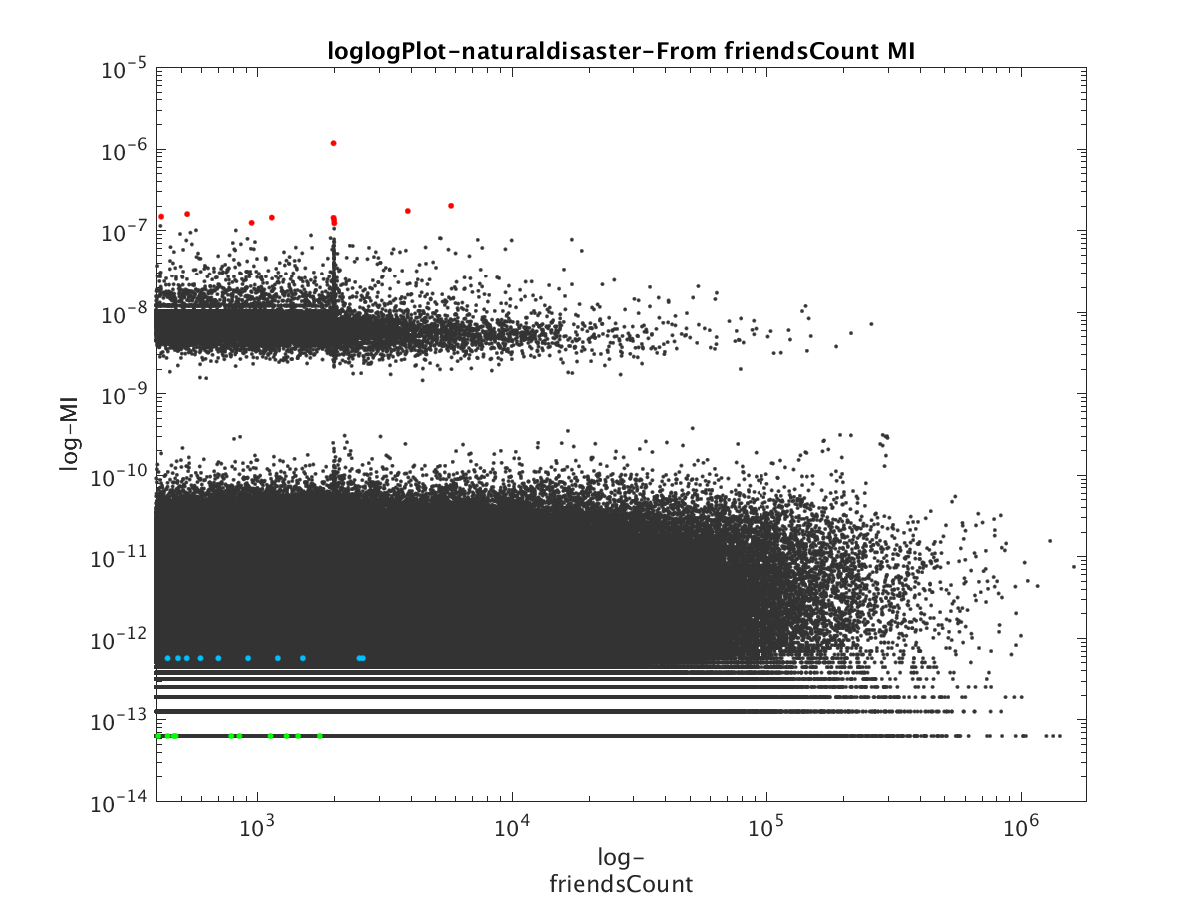
\epsfig{file=naturaldisaster-FromfriendsCountMI_log_log_Plot.png, height=2.5in, width=3in}
\caption{A sample scatter plot for Mutual Inforamtion of $FromUser$ vs. Friends Count (.eps format)
that has been resized with the \texttt{epsfig} command.}
\end{figure}

\begin{enumerate}
\item Anecdotal feature analysis: for each of 5 feature types: (rows) top-k / median-k (?), (cols) topics -- much better than below b/c we show all topics here and we can compare features across topics.

Don't use for now: show (rows) top-k and median-k features for different topics and (cols) 5 features (location, mention, from, term, hashtag) -- need to select a **few (2-3) interesting topics** and explain shown in table \ref{top10MItopicsLocations}

\item scatterplots of feature MI -- the absolute last thing we do (density plots?!!)

**which plots below, and for which topics?  Could pick out most useful features for topics in part (a)(i) and just show selected scatter plots below for these feature types.

from, mention MIs vs. {followers, favorites, friends, hashtags, tweets}

hashtag MI vs. {\#tweets, \#users}
location MI vs. {\#users}
term MI vs. {\#tweets}

\begin{figure}[h]
\centering
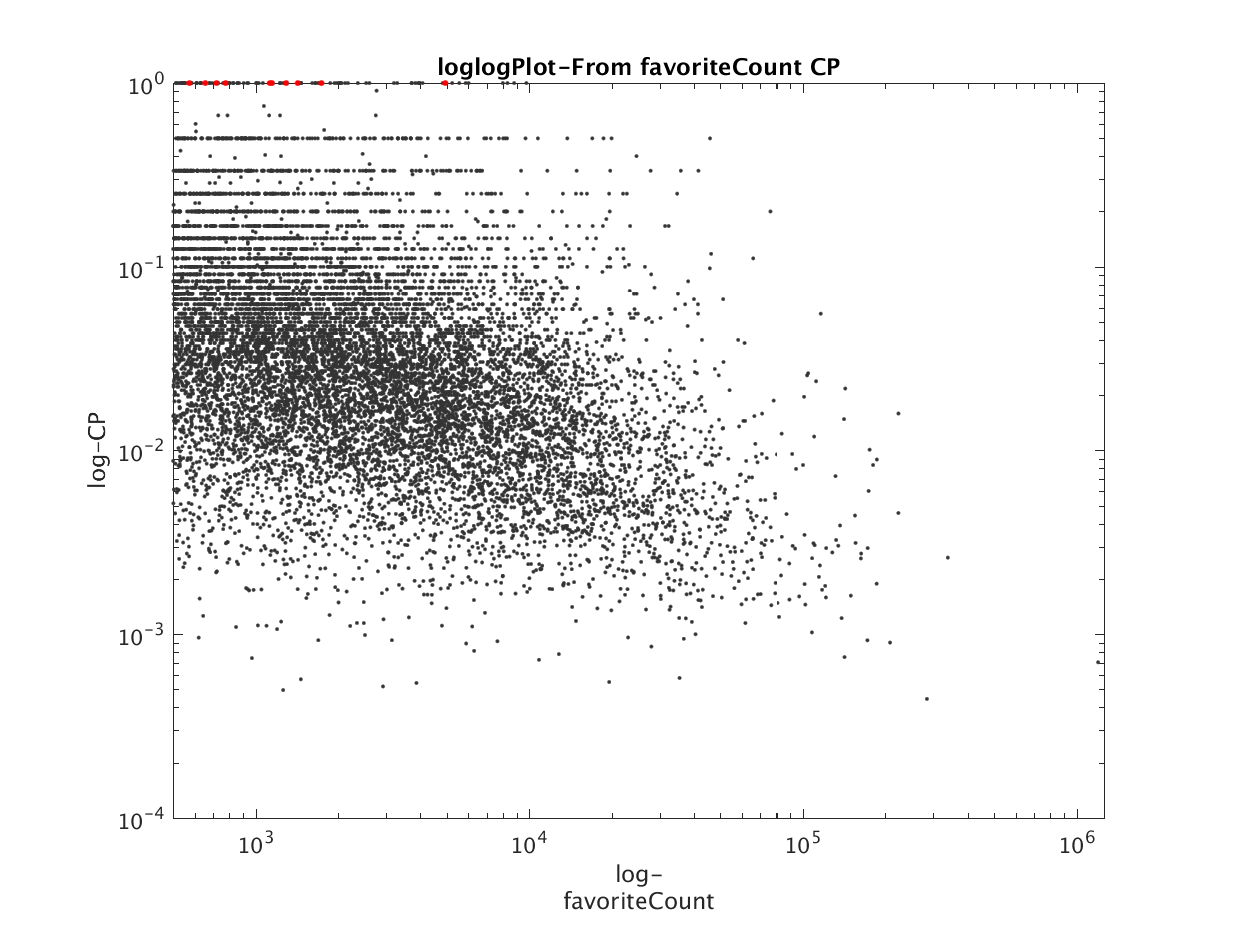
\epsfig{file=From_favoriteCount_CP_log_log_Plot.eps, height=2.5in, width=3in}
\caption{A sample scatter plot for Conditional Property of $FromUser$ vs. Favorite Count (.eps format)
that has been resized with the \texttt{epsfig} command.}
\end{figure}

\end{enumerate}

\end{itemize}

\section{Related Works}


\section{Conclusions}


%ACKNOWLEDGMENTS are optional
\section{Acknowledgments}
\cite{cuiZhang}

\section{Copyright}

\subsection{References} 
The aaai.sty file includes a set of definitions for use in formatting references with BibTeX. These definitions make the bibliography style fairly close to the one specified below. To use these definitions, you also need the BibTeX style file ``aaai.bst," available in the author kit on the AAAI web site. Then, at the end of your paper but before \textbackslash end{document}, you need to put the following lines:

\begin{quote}
\begin{small}
\textbackslash bibliographystyle\{aaai\}
\textbackslash bibliography\{bibfile1,bibfile2,...\}
\end{small}
\end{quote}

\end{document}
